\vspace{-0.3cm}
The results of the implemented methods from the previous chapter are documented in this section.
Statistics gathered from the data retrieval and dataset preparation methods, developed in~\ref{subsec:data-fetching}-\ref{subsec:sp_methods} chapters,
are recorded in the first results section~\ref{subsec:results_data}.
The performance metrics of ML models listed in chapter~\ref{subsec:ml_methods} are documented in section~\ref{subsec:machine_learning}.

\vspace{-0.2cm}

\subsection{Data Fetching and Feature Extraction}
\label{subsec:results_data}

The results section commences with the presentation of Table~\ref{tab:records}, which summarizes the data retrieval phase.
Displayed within are the total records obtained from both databases, along with the corresponding total and median values extracted.

\begin{table}[h]
    \renewcommand{\arraystretch}{1.5}
    \setlength{\tabcolsep}{12pt}
    \begin{center}
        \begin{tabular}{ |c|c|c| }
            \hline
            & MIMIC-III  & MIMIC-IV \\
            \hline
            Records       & 22,083     & 5,508    \\
            \hline
            Total Values  & 13,659,375 & 792,341  \\
            \hline
            Median Values & 1,918,623  & 110,408  \\
            \hline
        \end{tabular}
    \end{center}
    \vspace{-0.5cm}
    \captionsetup{format=plain, justification=centering}
    \caption{Fetched and Extracted Data from MIMIC-III and MIMIC-IV DBs}
    \label{tab:records}
\end{table}

\vspace{-0.5cm}
In a brief summary of the table data, 5,508 records were retrieved from the MIMIC-IV database, each encompassing 37,795 values, equating to approximately 605 seconds of data (at a sampling rate of 64.4725 Hz).
Conversely, a total of 22,083 records were obtained from the MIMIC-IV dataset, representing four times the number of records in comparison to MIMIC-IV\@.
Each of these records consisted of 75,625 values, likewise corresponding to an approximate duration of 10 minutes (with a sampling rate of 125 Hz).

Subsequently, the process of feature extraction from both DBs commenced, involving the extraction of 34 training features along with their corresponding values from the PPG waveforms,
as well as the target reference values for SBP, DBP, and MAP from the ABP signal.

From the MIMIC-IV dataset, a total of 792,341 values were extracted, leading to the creation of 34 x 792,341 PPG and 3 x 792,341 ABP data matrices.
Additionally, 110,408 median values were derived from these matrices, forming datasets of the same x-axis dimensions.
This set of data was utilized for the validation phase.

In the case of the MIMIC-III dataset, a total of 13,659,375 values were extracted, resulting in 34 x 13,659,375 PPG and 3 x 13,659,375 ABP data matrices.
Similarly, 1,918,623 median values were obtained from these matrices, creating datasets with identical X-axis structures.
These datasets were employed for the purposes of training and testing.

The data flow encompassing data retrieval, feature extraction and ML dataset creation is visualized in Figure~\ref{fig:data_flow}.

The performance metric for data fetching and feature extraction can be assessed by examining the average number of values extracted from each 10-minute record in the datasets.
In the case of MIMIC-IV, the calculation reveals an average of 143.85 values per record, derived from a total of 792,341 values extracted across 5,508 records.

\vspace{0.3cm}
\texttt{792,341 (total values) / 5,508 (records) = 143.85 values/record}
\vspace{0.3cm}

In contrast, for MIMIC-III, the average number of values per record is notably higher at 618.55, computed from a total of 13,659,375 values obtained from 22,083 records.

\vspace{0.3cm}
\texttt{13,659,375 (total values) / 22,083 (records) = 618.55 values/record}
\vspace{0.3cm}

These figures provide a quantitative measure of the efficiency and scale of data extraction from each dataset, with MIMIC-III yielding a substantially larger average number of extracted values per record
compared to MIMIC-IV, further discussed in the discussion section~\ref{subsec:ppg-feature-extraction}.

\vspace{1cm}
\begin{figure}[h]
    \centering
    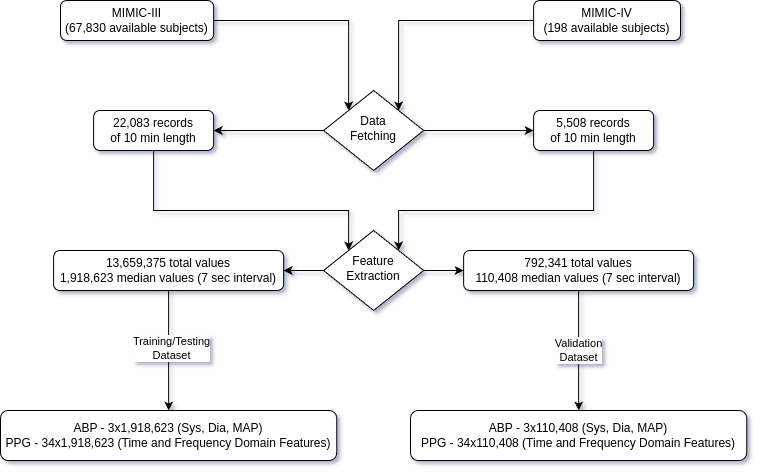
\includegraphics[width=\textwidth]{images/results/flow}
    \caption{A flow diagram presenting the data fetching and processing}
    \label{fig:data_flow}
\end{figure}

\newpage

\subsection{Machine Learning}
\label{subsec:machine_learning}

Moving forward to the results stemming from the ML phase, the initial focus lies on the preparation of feature data.

As outlined in previous chapters, the intended split ratio of 60/20/20 for train/test/validation could not be precisely achieved due to the final dataset sizes of 1,918,623 values from MIMIC-III and 110,408 values from MIMIC-IV\@.
Consequently, the MIMIC-III dataset was utilized for training and testing, being split into an 80/20 ratio for train/test, resulting in 1,534,898 training datapoints and 383,725 testing datapoints.
Thus, the ultimate distribution for train/test/validate proportions became:

\begin{center}
    \renewcommand{\arraystretch}{1.2}
    \setlength{\tabcolsep}{12pt}
    \begin{tabular}{|c|c|c|}
        \hline
        Training  & Testing & Validation \\
        \hline
        1,534,898 & 383,725 & 110,408    \\
        \hline
        76\%      & 19\%    & 5\%        \\
        \hline
    \end{tabular}
\end{center}

After implementing the 7 ML models outlined in the methods section~\ref{subsec:ml_methods} and employing the described training method with an \enquote{early stopping} strategy,
along with validation on unseen simulated \enquote{real-world} (MIMIC-IV) data, a comprehensive set of performance metrics was compiled.
Firstly, the training and testing losses, measured through MSE at the conclusion of training epochs, were documented.
Secondly, the overall testing accuracy was assessed using RMSE and MAE metrics.
Lastly, the validation loss, also utilizing RMSE and MAE, was computed.

All \textit{PyTorch} models were additionally executed alongside their \ac{WA} counterparts, with the respective metrics recorded.

The relevant ML model testing logs and performance metrics, including RMSE, MAE, \textit{$R^2$}, Bias and LoA are documented in Appendix~\ref{subsec:misc_measures}.

The plots depicting feature importance, along with their corresponding weight values from the second iteration of the ML models, are available in Appendix~\ref{subsec:plots_fi}.

The final results of all ML models for predicting ABP (SBP, DBP and MAP) are available in the Tables~\ref{tab:train_test_mse} and~\ref{tab:test_validate_rmse_mae}.
In the tables, the three highest and three lowest values of each column are color-coded.
A brighter shade of green indicates lower loss values, while a brighter shade of red indicates higher loss values.

The validated prediction accuracy of different BP measurements across all ML models is illustrated in the bar plot~\ref{fig:all_mae}.

\begin{table}[p]
    \thisfloatpagestyle{empty}
    \vspace{-2cm}
    \centering
    \begin{minipage}{\textwidth}
        \centering
        \renewcommand{\arraystretch}{1.5}
        \begin{tabular}{ |c|c|c| }
            \hline
            & Training Loss (MSE)        & Testing Loss (MSE)          \\
            \hline
            LR           & \cellcolor{red!10}217.673  & \cellcolor{red!10}217.255   \\
            \hline
            LR (WA)      & \cellcolor{red!20}217.721  & \cellcolor{red!20}217.284   \\
            \hline
            MLP          & 196.448                    & 196.158                     \\
            \hline
            MLP (WA)     & \cellcolor{red!30}246.247  & \cellcolor{red!30}249.776   \\
            \hline
            LSTM         & \cellcolor{green!20}97.452 & \cellcolor{green!20}101.49  \\
            \hline
            LSTM (WA)    & 138.708                    & 143.316                     \\
            \hline
            Bi-LSTM      & \cellcolor{green!10}115.1  & 118.12                      \\
            \hline
            Bi-LSTM (WA) & 154.553                    & 159.745                     \\
            \hline
            GRU          & \cellcolor{green!30}89.809 & \cellcolor{green!30}93.605  \\
            \hline
            GRU (WA)     & 138.081                    & 142.129                     \\
            \hline
            Bi-GRU       & 115.506                    & \cellcolor{green!10}117.732 \\
            \hline
            Bi-GRU (WA)  & 117.547                    & 173.893                     \\
            \hline
        \end{tabular}
        \captionsetup{format=plain, justification=centering, font=small}
        \vspace{-0.2cm}
        \caption{Training and Testing Losses of different ML models at the end of Training}
        \label{tab:train_test_mse}
        \vspace{0.2cm}
        \begin{tabular}{ |c|c|c|c|c| }
            \hline
            & Test MAE                  & Test RMSE                  & Validation MAE             & Validation RMSE            \\
            \hline
            LR           & \cellcolor{red!10}11.091  & \cellcolor{red!10}14.739   & \cellcolor{green!20}11.273 & \cellcolor{green!30}14.236 \\
            \hline
            LR (WA)      & \cellcolor{red!20}11.093  & \cellcolor{red!20}14.74    & \cellcolor{green!10}11.292 & \cellcolor{green!20}14.301 \\
            \hline
            MLP          & 10.567                    & 14.005                     & \cellcolor{green!30}11.072 & \cellcolor{green!10}14.737 \\
            \hline
            MLP (WA)     & \cellcolor{red!30}11.802  & \cellcolor{red!30}15.803   & \cellcolor{red!30}15.017   & \cellcolor{red!30}19.825   \\
            \hline
            LSTM         & \cellcolor{green!10}7.119 & \cellcolor{green!10}10.073 & \cellcolor{red!10}13.278   & \cellcolor{red!10}16.94    \\
            \hline
            LSTM (WA)    & 8.697                     & 11.971                     & 11.787                     & 14.94                      \\
            \hline
            Bi-LSTM      & 7.85                      & 10.868                     & \cellcolor{red!20}13.464   & \cellcolor{red!20}17.218   \\
            \hline
            Bi-LSTM (WA) & 9.362                     & 12.638                     & 12.063                     & 15.358                     \\
            \hline
            GRU          & \cellcolor{green!20}6.823 & \cellcolor{green!20}9.674  & 12.97                      & 16.62                      \\
            \hline
            GRU (WA)     & 8.658                     & 11.921                     & 12.062                     & 15.496                     \\
            \hline
            Bi-GRU       & 7.844                     & 10.85                      & 13.145                     & 16.645                     \\
            \hline
            Bi-GRU (WA)  & 9.811                     & 13.186                     & 11.614                     & 14.752                     \\
            \hline
            RF           & \cellcolor{green!30}5.075 & \cellcolor{green!30}8.148  & 12.457                     & 15.709                     \\
            \hline
        \end{tabular}
        \captionsetup{format=plain, justification=centering, font=small}
        \vspace{-0.2cm}
        \caption{Testing and Validation Performance Metrics of different ML Models}
        \label{tab:test_validate_rmse_mae}
    \end{minipage}
\end{table}

\newpage

\subsubsection{Feature Importance}
\label{subsubsec:feature_importance}

Based on the iterative evaluation approach described in the methods section, the feature importance values were systematically analysed, highlighting their impact on the model's performance.
The plots, available in the Appendix~\ref{subsec:plots_fi}, showcase these values in a descending order, revealing the features' contributions to either enhancing or diminishing the model's predictive power.
From the obtained results, a portion of the features can be categorized into three groups based on their average importance values.

In the category of best performers, features such as
\begin{itemize}[itemsep=2pt]
    \item Diastolic Time (86.89),
    \item Resistive Index (67.31),
    \item Diastolic + Systolic Width at 50\% (50.6) and
    \item Normalized Power at Peak (46.72)
\end{itemize}
stood out prominently, demonstrating significant influence in improving the models' accuracy.

In the medium-performing group, features like
\begin{itemize}[itemsep=2pt]
    \item Delta Area (37.12),
    \item Vessel Volume Systolic Index (23.61),
    \item Systolic Area and
    \item Total Power (both with values of 20.79), also
    \item Diastolic Width at 66\% (17.66) and
    \item Vessel Volume Diastolic Index (14.27),
\end{itemize}
contributed moderately to the overall predictive capability.

Lastly, in the category of least influential features
\begin{itemize}[itemsep=2pt]
    \item Mean Frequency (3.51)
    \item and Ratio of Diastolic to Systolic Width at 75\% (2.12)
\end{itemize}
showed minimal impact on the models' performance.

\subsubsection{Model Performance}
\label{subsubsec:model_performance}

The results of the Machine Learning models, as summarized in Table~\ref{tab:train_test_mse} , reveal varying levels of performance in terms of training and testing losses (calculated as MSE) at the conclusion of training epochs.
The intermediate training and testing losses are plotted in Figure~\ref{fig:train_test_mse}.

\vspace{0.2cm}
\textit{Training and Testing Loss}
\vspace{0.2cm}

The LR model exhibited a training loss of 217.673 and a testing loss of 217.255, with marginal improvement seen in the WA version.
Similarly, the MLP model showed a training loss of 196.448 and a testing loss of 196.158, with a notable increase in losses for the WA variant.

On the other hand, the LSTM model demonstrated improved performance, showcasing a training loss of 97.452 and a testing loss of 101.49, while the Bi-LSTM and Bi-GRU models also exhibited relatively lower losses.
The GRU model, in particular, displayed a training loss of 89.809 and a testing loss of 93.605, indicating promising results for this configuration.

Overall, the models' performances varied, with some showing better generalization capabilities than others, as evident from their testing losses.

\vspace{0.2cm}
\textit{Testing and Validation Performance}
\vspace{0.2cm}

The Table~\ref{tab:test_validate_rmse_mae} provides an overview of the testing and validation performance metrics for the Machine Learning models employed.

For the LR model, the test MAE and RMSE were recorded as 11.091 and 14.739 respectively, with the validation MAE at 11.273 and RMSE at 14.236.
Similarly, the LR WA model exhibited comparable metrics with slightly higher validation MAE and RMSE values.
The LR model demonstrated among the least favorable testing results, yet it displayed some of the most favorable validation metrics.

Moving to the MLP model, it displayed a test MAE of 10.567 and a test RMSE of 14.005, with the validation metrics showing an MAE of 11.072 and RMSE of 14.737.
The MLP WA model significantly increased both testing and validation MAE and RMSE values to 15.017 and 19.825 respectively, displaying the worst performance of all models.
Nonetheless, the unadjusted MLP model exhibited the absolute best validation MAE among all models and ranked within the top three for validation RMSE\@.

\newpage
In contrast, the LSTM model displayed enhanced performance with a test MAE of 7.119 and a test RMSE of 10.073, while its WA version did not improve the testing performance.
The validation metrics for the LSTM model were recorded as an MAE of 13.278 and an RMSE of 16.94, ranking among the lowest performers.
However, during validation, the WA LSTM model notably enhanced both its MAE and RMSE\@.

The Bi-LSTM model demonstrated comparatively lower MAE and RMSE values for the test set compared to the LSTM model, but it notably underperformed in validation, making it the second lowest-ranking model in terms of validation MAE and RMSE\@.
However, the WA adjusted version exhibited less efficiency during testing yet displayed improvements during validation.

The GRU model displayed a test MAE of 6.823 and a test RMSE of 9.674, the best scores out of all PyTorch models, with the validation MAE at 12.97 and RMSE at 16.62.
The weight adjustment likewise reduced its testing performance while enhancing its validation performance.

For the Bi-GRU model, the test MAE and RMSE were 7.844 and 10.85, while the validation MAE and RMSE were recorded as 13.145 and 16.645 respectively.
Once again, the WA versions notably improved the validation metrics, nearly approaching the LR and MLP metrics with its 11.614 validation MAE\@.

Lastly, the RF model stood out with the lowest test MAE and RMSE of 5.075 and 8.148 respectively.
The validation MAE for RF was 12.457 and RMSE was 15.709.
Even though the RF model demonstrated robust predictive accuracy on the testing dataset, it only achieved average metrics for the validation dataset.

The analysis reveals varying performances across the models, with RF emerging as the strongest performer during testing, by displaying the lowest values for both MAE and RMSE\@.
Conversely, the top performers in validation were MLP, achieving the best MAE, and LR, showcasing the best RMSE among all models.

\newpage

\subsubsection{Prediction Performance of different BP measurements}
\label{subsubsec:bp_prediction_performance}

For the final evaluation of performance, the average, best, and worst validation MAE values were computed and visualized in Figure~\ref{fig:all_mae}.

\begin{figure}[h]
    \centering
    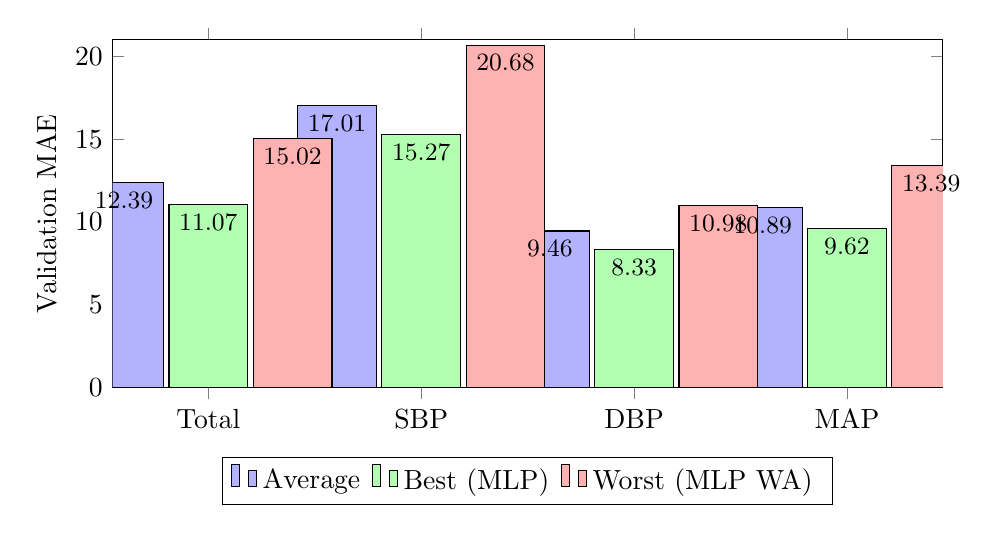
\begin{tikzpicture}
        \begin{axis}[
            width=\textwidth,
            height=6cm,
            ybar,
            ymin=0,
            ymax=21,
            bar width=1cm,
            xtick=data,
            xticklabels={Total, SBP, DBP, MAP},
            x tick label style={/pgf/number format/1000 sep=},
            enlarge x limits=0.15,
            ylabel={Validation MAE},
            nodes near coords,
            nodes near coords style={font=\small, anchor=north, /pgf/number format/.cd, fixed, precision=2},
            legend style={at={(0.5,-0.2)}, anchor=north, legend columns=-1},
        ]
            \addplot[fill=blue!30] coordinates {(1,12.392) (2,17.012) (3,9.457) (4,10.887)};
            \addlegendentry{Average\:}
            \addplot[fill=green!30] coordinates {(1,11.07) (2,15.273) (3,8.328) (4,9.616)};
            \addlegendentry{Best (MLP)\:}
            \addplot[fill=red!30] coordinates {(1,15.017) (2,20.675) (3,10.983) (4,13.393)};
            \addlegendentry{Worst (MLP WA)\:}
        \end{axis}
    \end{tikzpicture}
    \captionsetup{format=plain, justification=centering, font=small}
    \caption{Average validation MAE of total, systolic, diastolic and mean arterial pressures}
    \label{fig:all_mae}
\end{figure}

This bar plot summarizes the average validation MAE for one overall and three distinct BP measurements, also providing the $\sigma$ values in brackets.
The plot compares the overall average MAE across all models, denoted in blue, showing a value of 12.392 ($\sigma$=10.05).

Additionally, it highlights the best-performing model in green, represented by the best (MLP) category, with MAE values of 11.07 ($\sigma$=9.725) for Total,
15.273 ($\sigma$=13045) for SBP, 8.328 ($\sigma$=5.814) for DBP, and 9.616 ($\sigma$=7.243) for MAP\@.

Conversely, the worst-performing model, indicated in red as Worst (MLP WA), exhibits higher MAE values across the board, with 15.017 ($\sigma$=12.944) for Total,
20.675 ($\sigma$=16.705) for SBP, 10.983 ($\sigma$=8.14) for DBP, and 13.393 ($\sigma$=10.312) for MAP\@.

This visualization provides a comparative overview of the model performances, with the best (MLP) model demonstrating the lowest MAE across all BP measurements,
followed by the overall average and the worst (MLP WA) model with the highest MAE values.

\begin{figure}[p]
    \thisfloatpagestyle{empty}
    \centering
    \begin{minipage}{\textwidth}
        \vspace{-2cm}
        \centering
        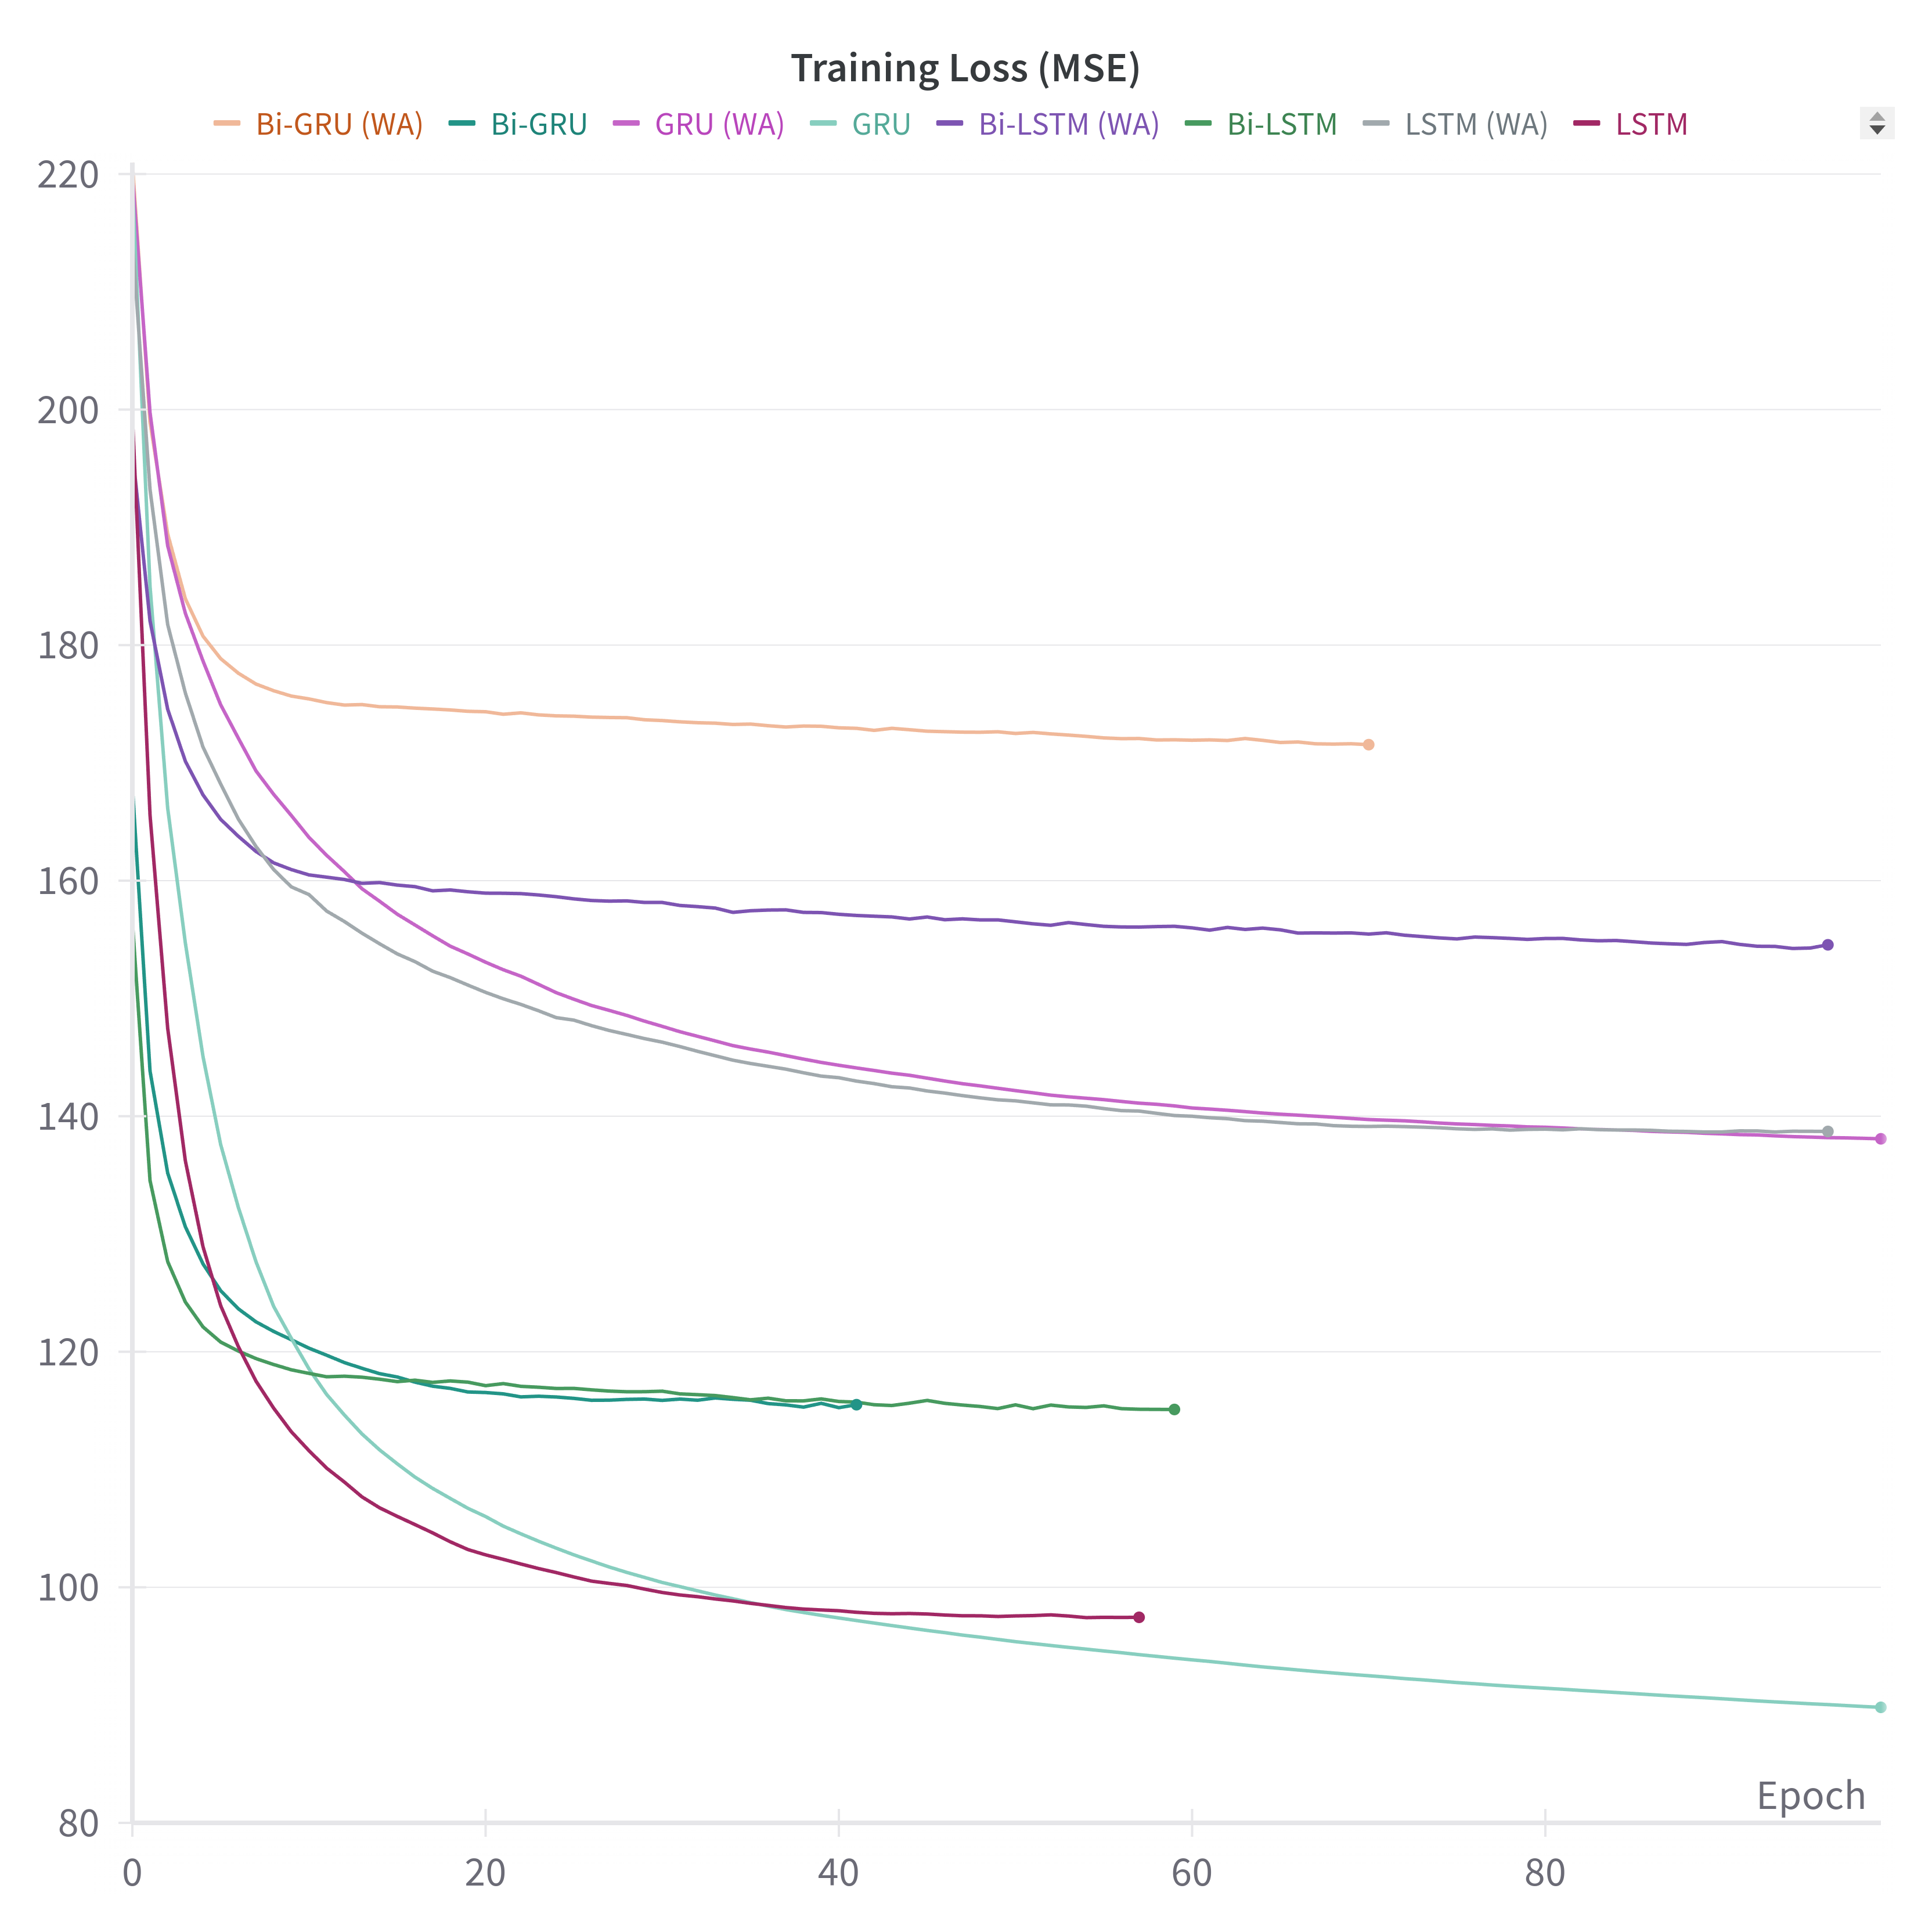
\includegraphics[width=0.9\textwidth]{images/results/training_loss_mse}
        \vspace{0.001cm}
        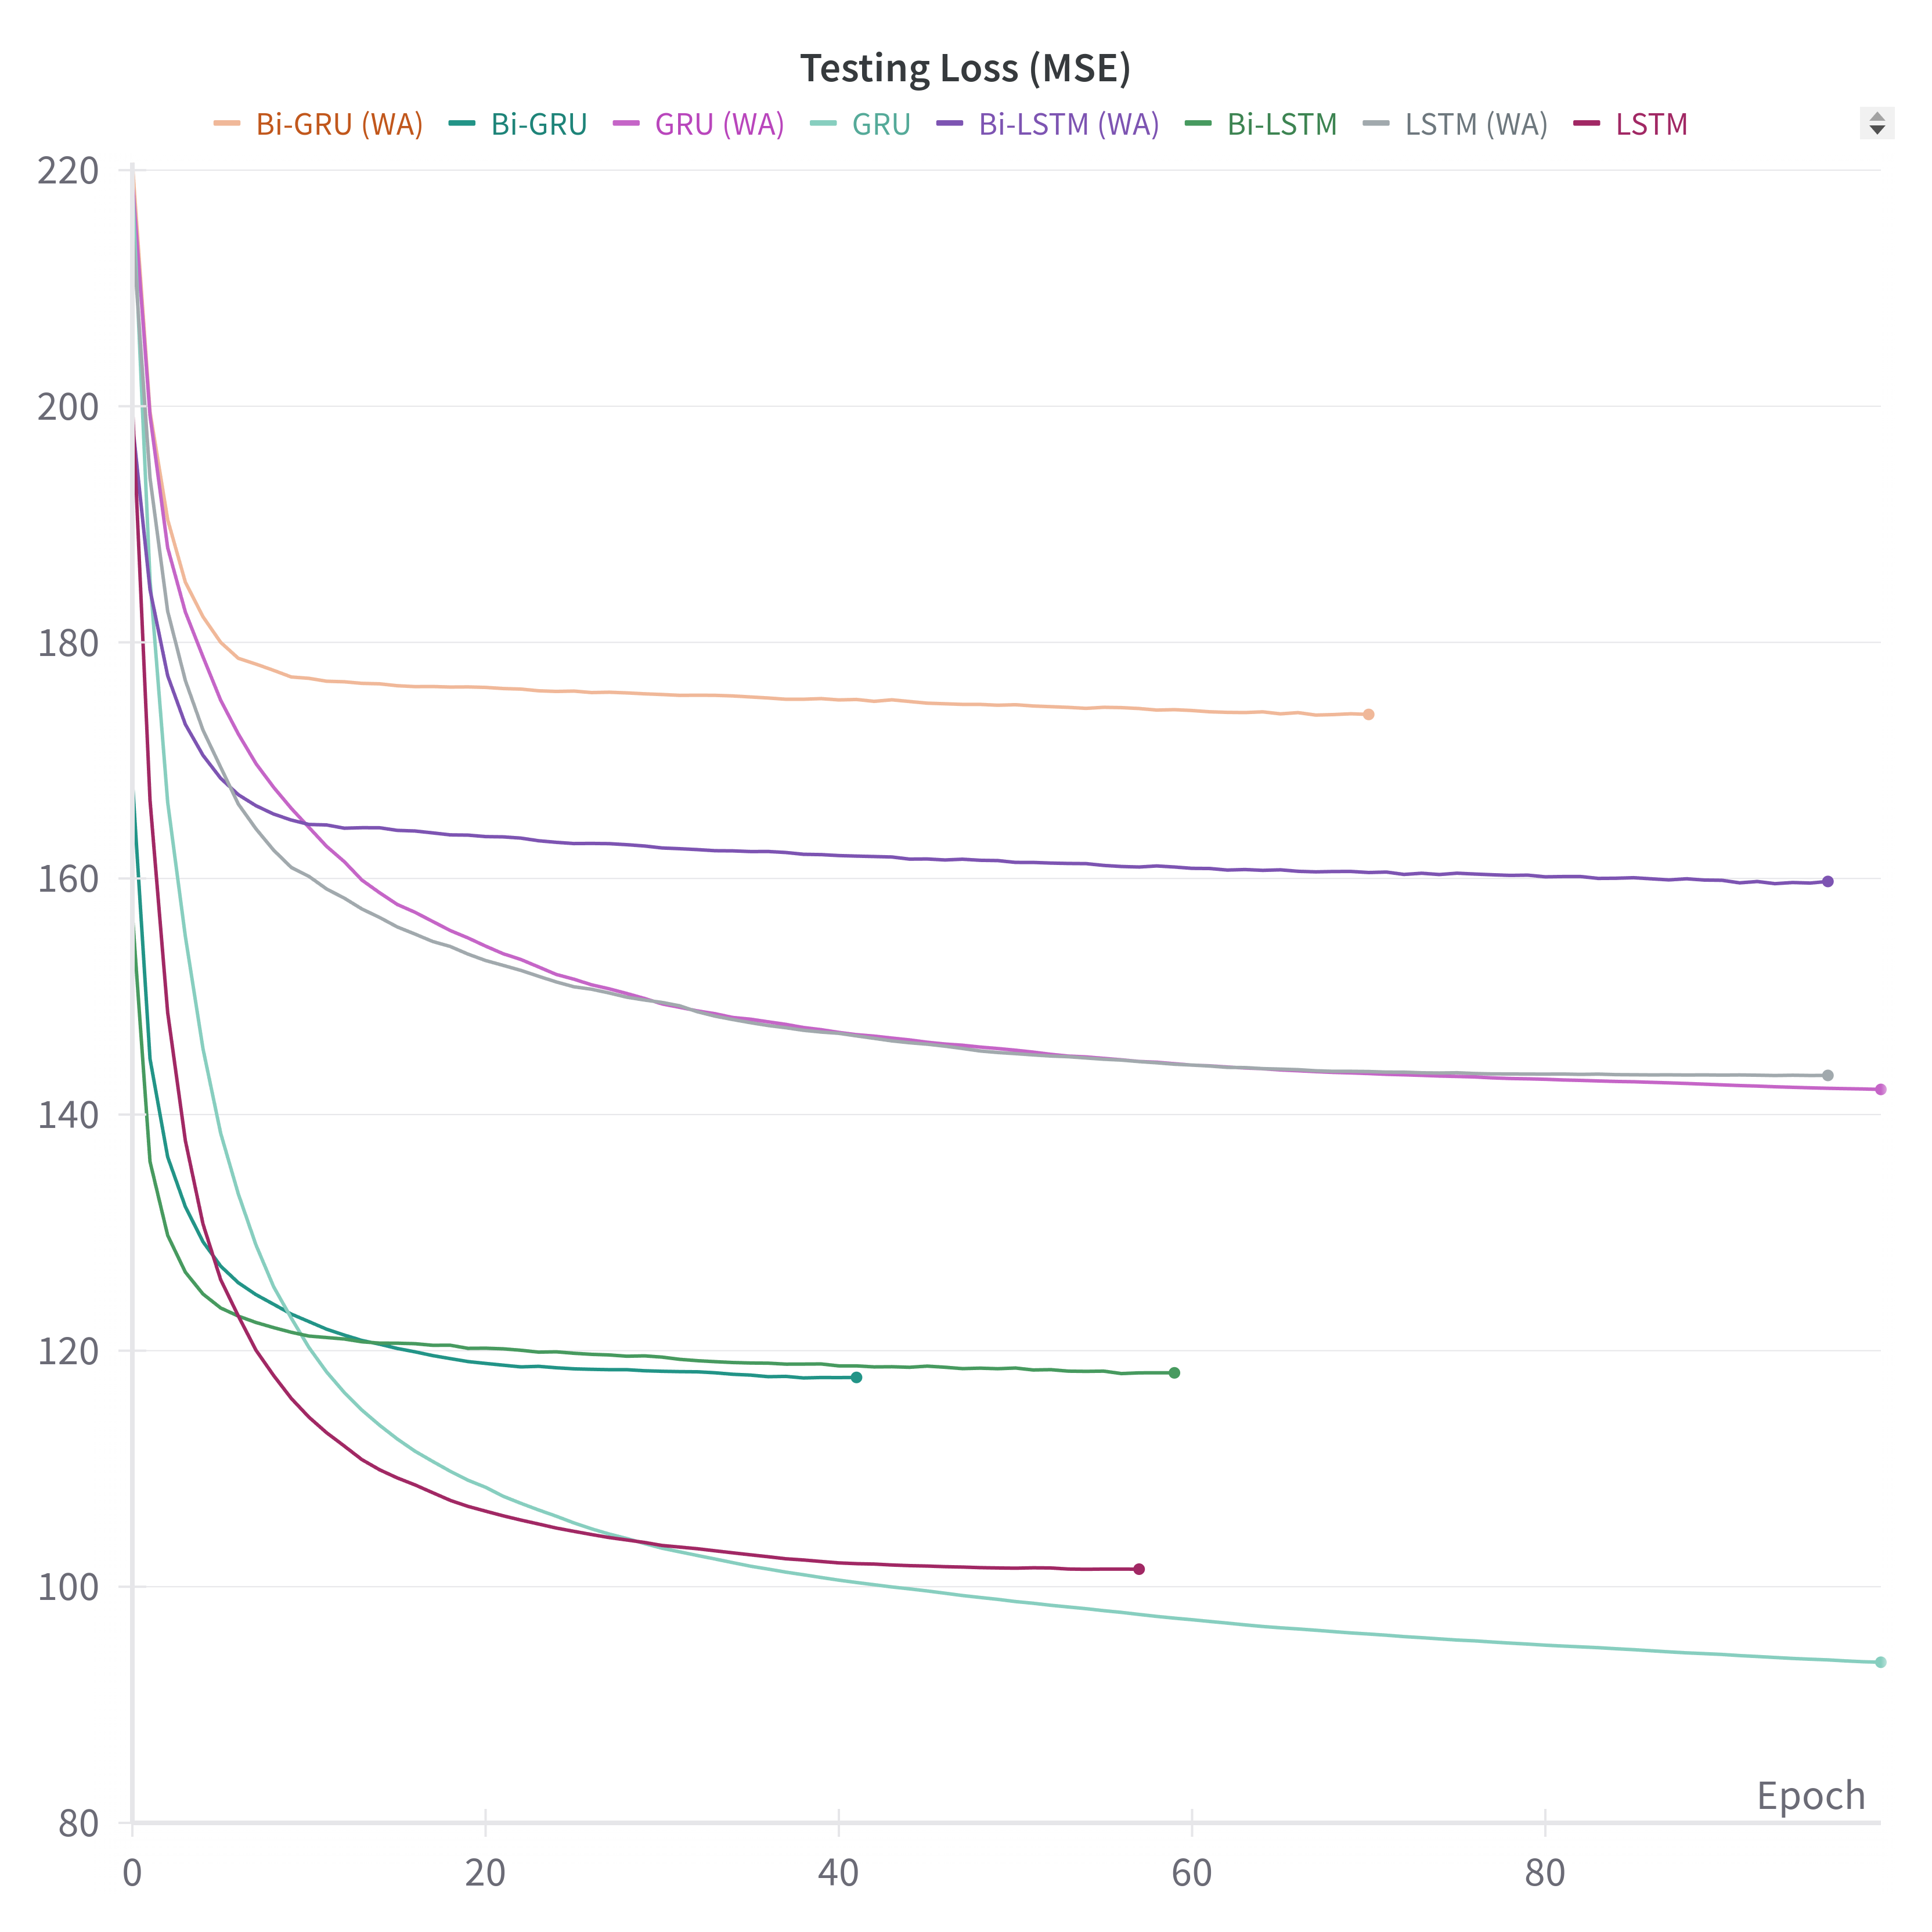
\includegraphics[width=0.9\textwidth]{images/results/testing_loss_mse}
        \captionsetup{format=plain, justification=centering, font=small}
        \vspace{-0.5cm}
        \caption{Training and Testing Losses of LSTM \& GRU Models}
        \label{fig:train_test_mse}
    \end{minipage}
\end{figure}

\newpage